% *==================================================================================*
% *                     Review vs. Camera-Ready settings                             *
% *==================================================================================*
%
% REVIEW: Use the following command for submitting the paper (double-blind,
% for review):
% \documentclass{Interspeech}
%
% CAMERA-READY: Use the following command for the camera-ready version, one
% affiliation per line:
\documentclass[cameraready]{Interspeech}
% *==================================================================================*

\usepackage{amsmath,graphicx,hyperref}

\usepackage{cite}
\usepackage{newtxmath}
\usepackage{booktabs,multirow}

% **************************************
% *                                    *
% *      STOP !   DO NOT DELETE !      *
% *          READ THIS FIRST           *
% *                                    *
% * This template also includes        *
% * important INSTRUCTIONS that you    *
% * must follow when preparing your    *
% * paper. Read it BEFORE replacing    *
% * the content with your own work.    *
% **************************************

%==================================================================================
% Title
% Must exactly match the title entered into the paper submission system
\title{A Large-Scale Probing Analysis of Speaker-Specific Attributes in Self-Supervised Speech Representations}

%==================================================================================
% Authors
% The order of authors here must exactly match the order entered into the paper submission system
% Note that the COMPLETE list of authors MUST be entered into the paper submission system at the outset, including when submitting your manuscript for double-blind review
% The ORCID number is still optional but will become mandatory in the future years. It is strongly encouraged to get an ORCID for each cu-author.
% Middle names, including initials, must be included in the first name
\author[affiliation={\ddagger}, orcid=0009-0005-9672-8147]{Aemon Yat Fei}{Chiu}
\author[affiliation={\ddagger}, orcid=0009-0007-2058-4831]{Kei Ching}{Fung}
\author[affiliation={\ddagger}, orcid=0009-0002-1829-0344]{Roger Tsz Yeung}{Li}
\author[affiliation={\dagger}, orcid=0000-0001-5617-7014]{Jingyu}{Li}
\author[affiliation={\ddagger,\diamond}, orcid=0000-0002-7089-3436]{Tan}{Lee}
% The maximum number of authors in the author list is 20. If the number of contributing authors is more than this, they should be listed in a footnote or the acknowledgement section.

%==================================================================================
% Affiliations

\address{
    $^{\ddagger}$ Department of Electronic Engineering, The Chinese University of Hong Kong, Hong Kong \\
    $^{\dagger}$ Independent Researcher \\
    $^{\diamond}$ School of Data Science, The Chinese University of Hong Kong, Shenzhen, China
}

%==================================================================================
% Emails
\email{\{aemon.yf.chiu,pacokcfung,rogerli,lijingyu0125\}@link.cuhk.edu.hk, tanlee@ee.cuhk.edu.hk}

%==================================================================================
% Keywords
\keywords{speech representation learning, speaker-specific attribute, probing, explainable AI.}

\newcommand{\blue}[1]{\textcolor{blue}{#1}}
\newcommand{\red}[1]{\textcolor{red}{#1}}
\newcommand{\best}[1]{\textbf{#1}}
\usepackage{comment}

%==================================================================================
% Content

\begin{document}

\maketitle

% the abstract here must exactly match the abstract entered into the paper submission system
\begin{abstract}
    % 1000 characters. ASCII characters only. No citations.
    Enhancing explainability in speech self-supervised learning (SSL) is important for developing reliable SSL-based speech processing systems. This study probes how speech SSL models encode speaker-specific information via a large-scale probing analysis of 11 models, decomposing identity into acoustic, prosodic, and paralinguistic attributes. The results confirm a general hierarchy wherein initial layers encode fundamental acoustics and middle layers synthesise abstract traits. Crucially, the consensus that final layers purely abstract linguistic content is challenged. It is discovered that larger models unexpectedly recover speaker identity in their deep layers. Furthermore, the intermediate representations of speech SSL models are found to capture dynamic prosody better than specialised speaker embeddings. These insights decode the complex internal mechanics of SSL models, providing guidelines for selecting interpretable and task-optimal representations.
\end{abstract}



\section{Introduction}
\label{sec:intro}

Speech representation learning has rapidly advanced in recent years~\cite{ssl, yang2024taslp, wang2024taslp}, driven by the success of large-scale Transformer-based \cite{attention} speech self-supervised learning (SSL) models such as Wav2vec 2.0~\cite{wav2vec2}, HuBERT~\cite{hubert}, UniSpeech-SAT~\cite{unispeech-sat}, and WavLM~\cite{wavlm}. These models have transformed speech representation learning by extracting rich and hierarchical representations from massive amounts of unlabelled audio, achieving state-of-the-art performance on a wide range of generalised downstream tasks. Typical speech SSL models generally comprise a convolutional neural network (CNN) encoder and a series of Transformer layers, as illustrated in Figure~\ref{fig:ssl}~\cite{wav2vec2, hubert, unispeech-sat, wavlm}. Nevertheless, like other models based on deep neural networks (DNN), these speech SSL models essentially operate as complex black boxes. Understanding their internal mechanics is significant for their effective utilisation. It is accepted that the lower layers of these models capture acoustic details, while the upper layers abstract linguistic content~\cite{ssl, yang2024taslp}. However, this high-level view does not fully capture the complexity of the information encoded, particularly regarding the varied nature of a speaker's voice.

Human communication is not a direct mapping from sound to words. Rather, it is a complex informational signal that can be decomposed into distinct streams. Prior work in phonetics~\cite{semiotic} and modern text-to-speech synthesis (TTS)~\cite{SpeechTripleNet,gengembre24_interspeech} distinguishes between the timbre, linguistic content, and prosody. Understanding how speech SSL models manage these distinct attributes is crucial for improving interpretability and developing more reliable downstream applications.

This study serves as a comprehensive explainability analysis and is motivated by the following research questions: \textbf{how do speech SSL models disentangle and represent different categories of speaker-specific attributes across their layers, and how do various model families and scales differ in encoding these attributes?} While previous studies have investigated various acoustic and linguistic properties encoded in deep speaker embeddings \cite{wang17g_Interspeech, raj19asru} and speech SSL representations \cite{pasad2021asru, pasad2023icassp, choi24b_interspeech, singla2022icdmw, Ashihara}, this study is the first to systematically investigate a curated set of speaker-specific attributes encoded across a wide range of speech SSL models and variants. By framing the analysis of continuous attributes as a classification task with discretised labels, a more direct and intuitive comparison across models is conducted. This approach facilitates an understanding of how these large models learn to separate the dynamic and stylistic elements of speech, giving practical implications for model selection in downstream tasks.


\begin{figure}[t]
  \centering
  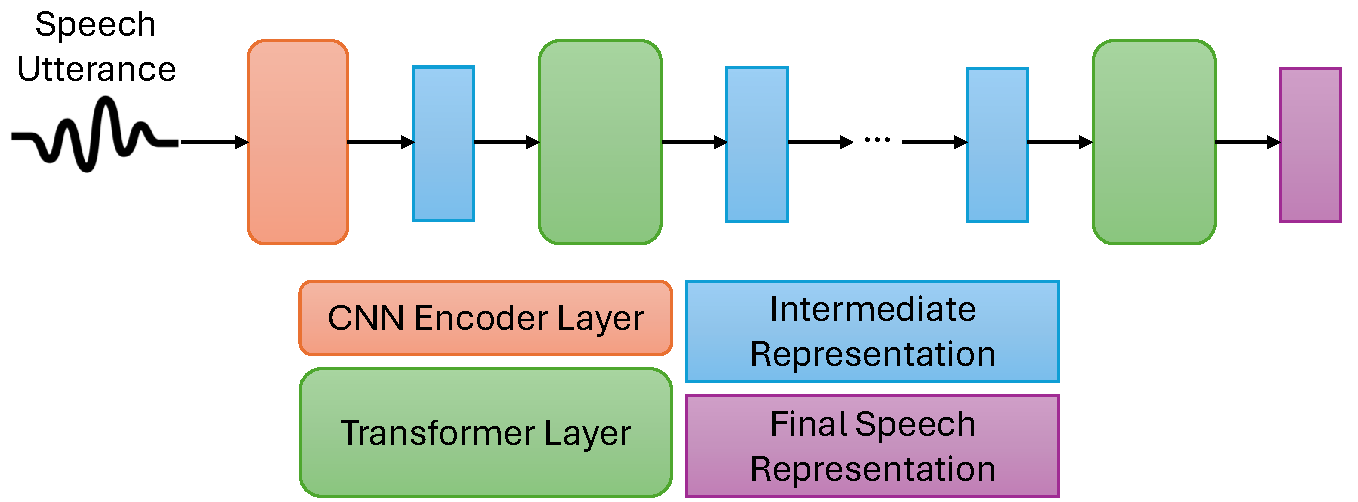
\includegraphics[width=0.95\linewidth]{figures/ssl.pdf}
  \vspace{-0.75em}
  \caption{A schematic diagram of typical speech SSL models~\cite{wav2vec2, hubert, unispeech-sat, wavlm}.}
\label{fig:ssl}
\vspace{-1.85em}
\end{figure}



\section{Related Work}
\label{sec:review}

\subsection{Probing single-vector deep speaker embeddings}
\label{sec:review_dse}

The use of simple classifiers to ``probe'' the information contained in learnt representations was established in foundational studies of deep speaker embeddings (e.g., $i$-vectors, $d$-vectors, and $s$-vectors), examining whether they capture fine-grained speaker attributes like gender and speaking rate~\cite{wang17g_Interspeech}. Raj et al. \cite{raj19asru} extended this to $x$-vectors, where they also analysed the model's robustness to data augmentation.

While prior work demonstrated that speaker embeddings trained for speaker verification (SV) also captured many other attributes, including speaking rate, gender, and linguistic content, the present study extends the probing paradigm to the latest Transformer-based speech SSL models, focusing on the evolution of the information across layers.


\begin{figure}[t]
  \centering
  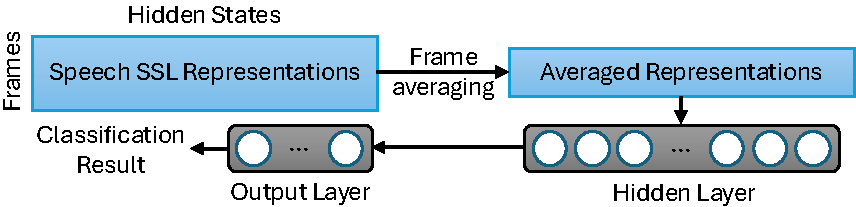
\includegraphics[width=\linewidth]{figures/probing_v2.pdf}
  \vspace{-2em}
  \caption{The overall design of the probing task for speech SSL representations.}
\label{fig:probing}
\vspace{-1.85em}
\end{figure}



\subsection{Layer-wise analysis of speech SSL models}
\label{sec:review_ssl}

Recent research has provided extensive analyses of speech SSL models, employing a range of methodologies and focusing on different aspects of speech. Canonical correlation analysis was used in \cite{pasad2021asru, pasad2023icassp} to map the layer-wise distribution of acoustic, phonetic, and word-level information, revealing how it is shaped by a model's pre-training objective. A subsequent study \cite{choi24b_interspeech} used direct similarity metrics to show that speech SSL representations are more sensitive to phonetic similarity than semantic similarity.

Singla et al. \cite{singla2022icdmw} comprehensively probed an extensive set of 46 features related to language delivery and structure, creating a detailed inventory of what is learnt in each layer. Ashihara et al. \cite{Ashihara} used probing tasks to compare the capabilities of general-purpose speech SSL models against specialised speaker SSL models, finding that the former retain more linguistic information while the latter are more capable of capturing speaker identity. The present study is distinct from the literature in its conceptual framework and analytical scope by employing a concisely grouped set of speaker-specific acoustic and prosodic attributes derived from phonetic literature, and by covering a wider range of model families and variants.




\section{Experimental Settings}

The probing method is based on an intuitive idea that well-encoded information in a speaker representation should enable a simple classifier to accurately identify that specific information accurately \cite{wang17g_Interspeech}. Accordingly, the probing pipeline is constructed as illustrated in Figure \ref{fig:probing}.


\subsection{Probing network}

Following the classifier designed in~ \cite{wang17g_Interspeech,raj19asru}, a simple classification network, i.e., a multilayer perceptron (MLP), is utilised as the probing model. The MLP has a single hidden layer with $500$ nodes followed by a ReLU activation. The input size of the MLP corresponds to the number of hidden states in the speech SSL representations, as these representations are frame-averaged before being fed into the MLP.





\subsection{Dataset}
\label{sec:dataset}

The TextrolSpeech dataset \cite{ji2024icassp} is used for the training and test datasets in the probing tasks. TextrolSpeech is a large-scale dataset comprising over 330 hours of English speech data with rich labels for controllable TTS. It integrates LibriTTS \cite{zen19_interspeech}, VCTK \cite{vctk}, and emotional TTS datasets, including ESD \cite{ZHOU20221ESD}, TESS \cite{tess}, MEAD \cite{mead}, SAVEE \cite{savee}, and MESS \cite{mess}. These last five emotional datasets make up 16\% of the corpus and contain labels for gender, pitch, tempo, energy, and emotion. LibriTTS and VCTK also are also enriched with these labels, although their emotion are labelled as ``Neutral''. A total of 1,327 speakers are included in the dataset, which is partitioned into training and test sets. In this study, 90\% of each subset of the original TextrolSpeech training set is randomly sampled to form the training set, totalling 212,400 utterances, while the remaining 10\% (23,603 samples) forms the validation set. Following training and validation, the MLP is evaluated on a test set containing 200 utterances, which is identical to the test set in the original TextrolSpeech dataset.

\begin{figure}[t]
  \centering
  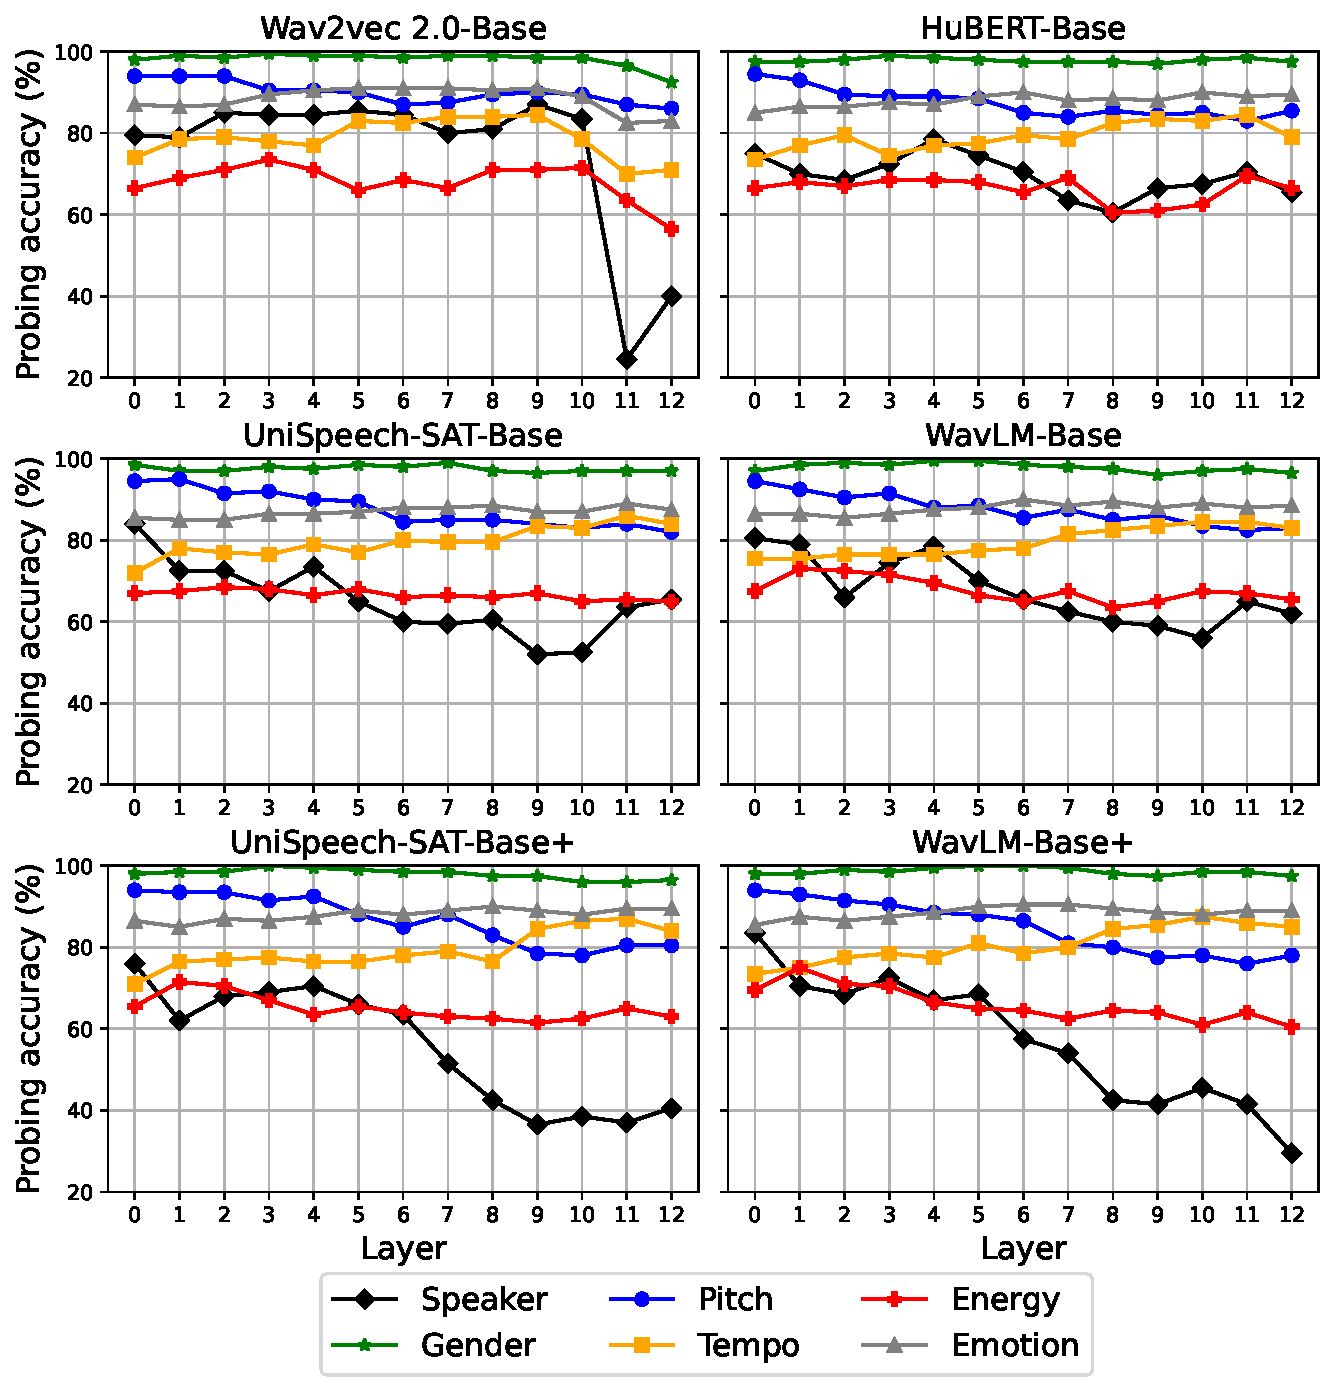
\includegraphics[width=\linewidth]{figures/Fig3.pdf}
  \vspace{-2em}
  \caption{Probing accuracies for the \textit{Base} and \textit{Base Plus} variants of speech SSL models on the test set.}
\label{fig:base}
\vspace{-1.85em}
\end{figure}


\begin{figure*}[t!]
  \centering
  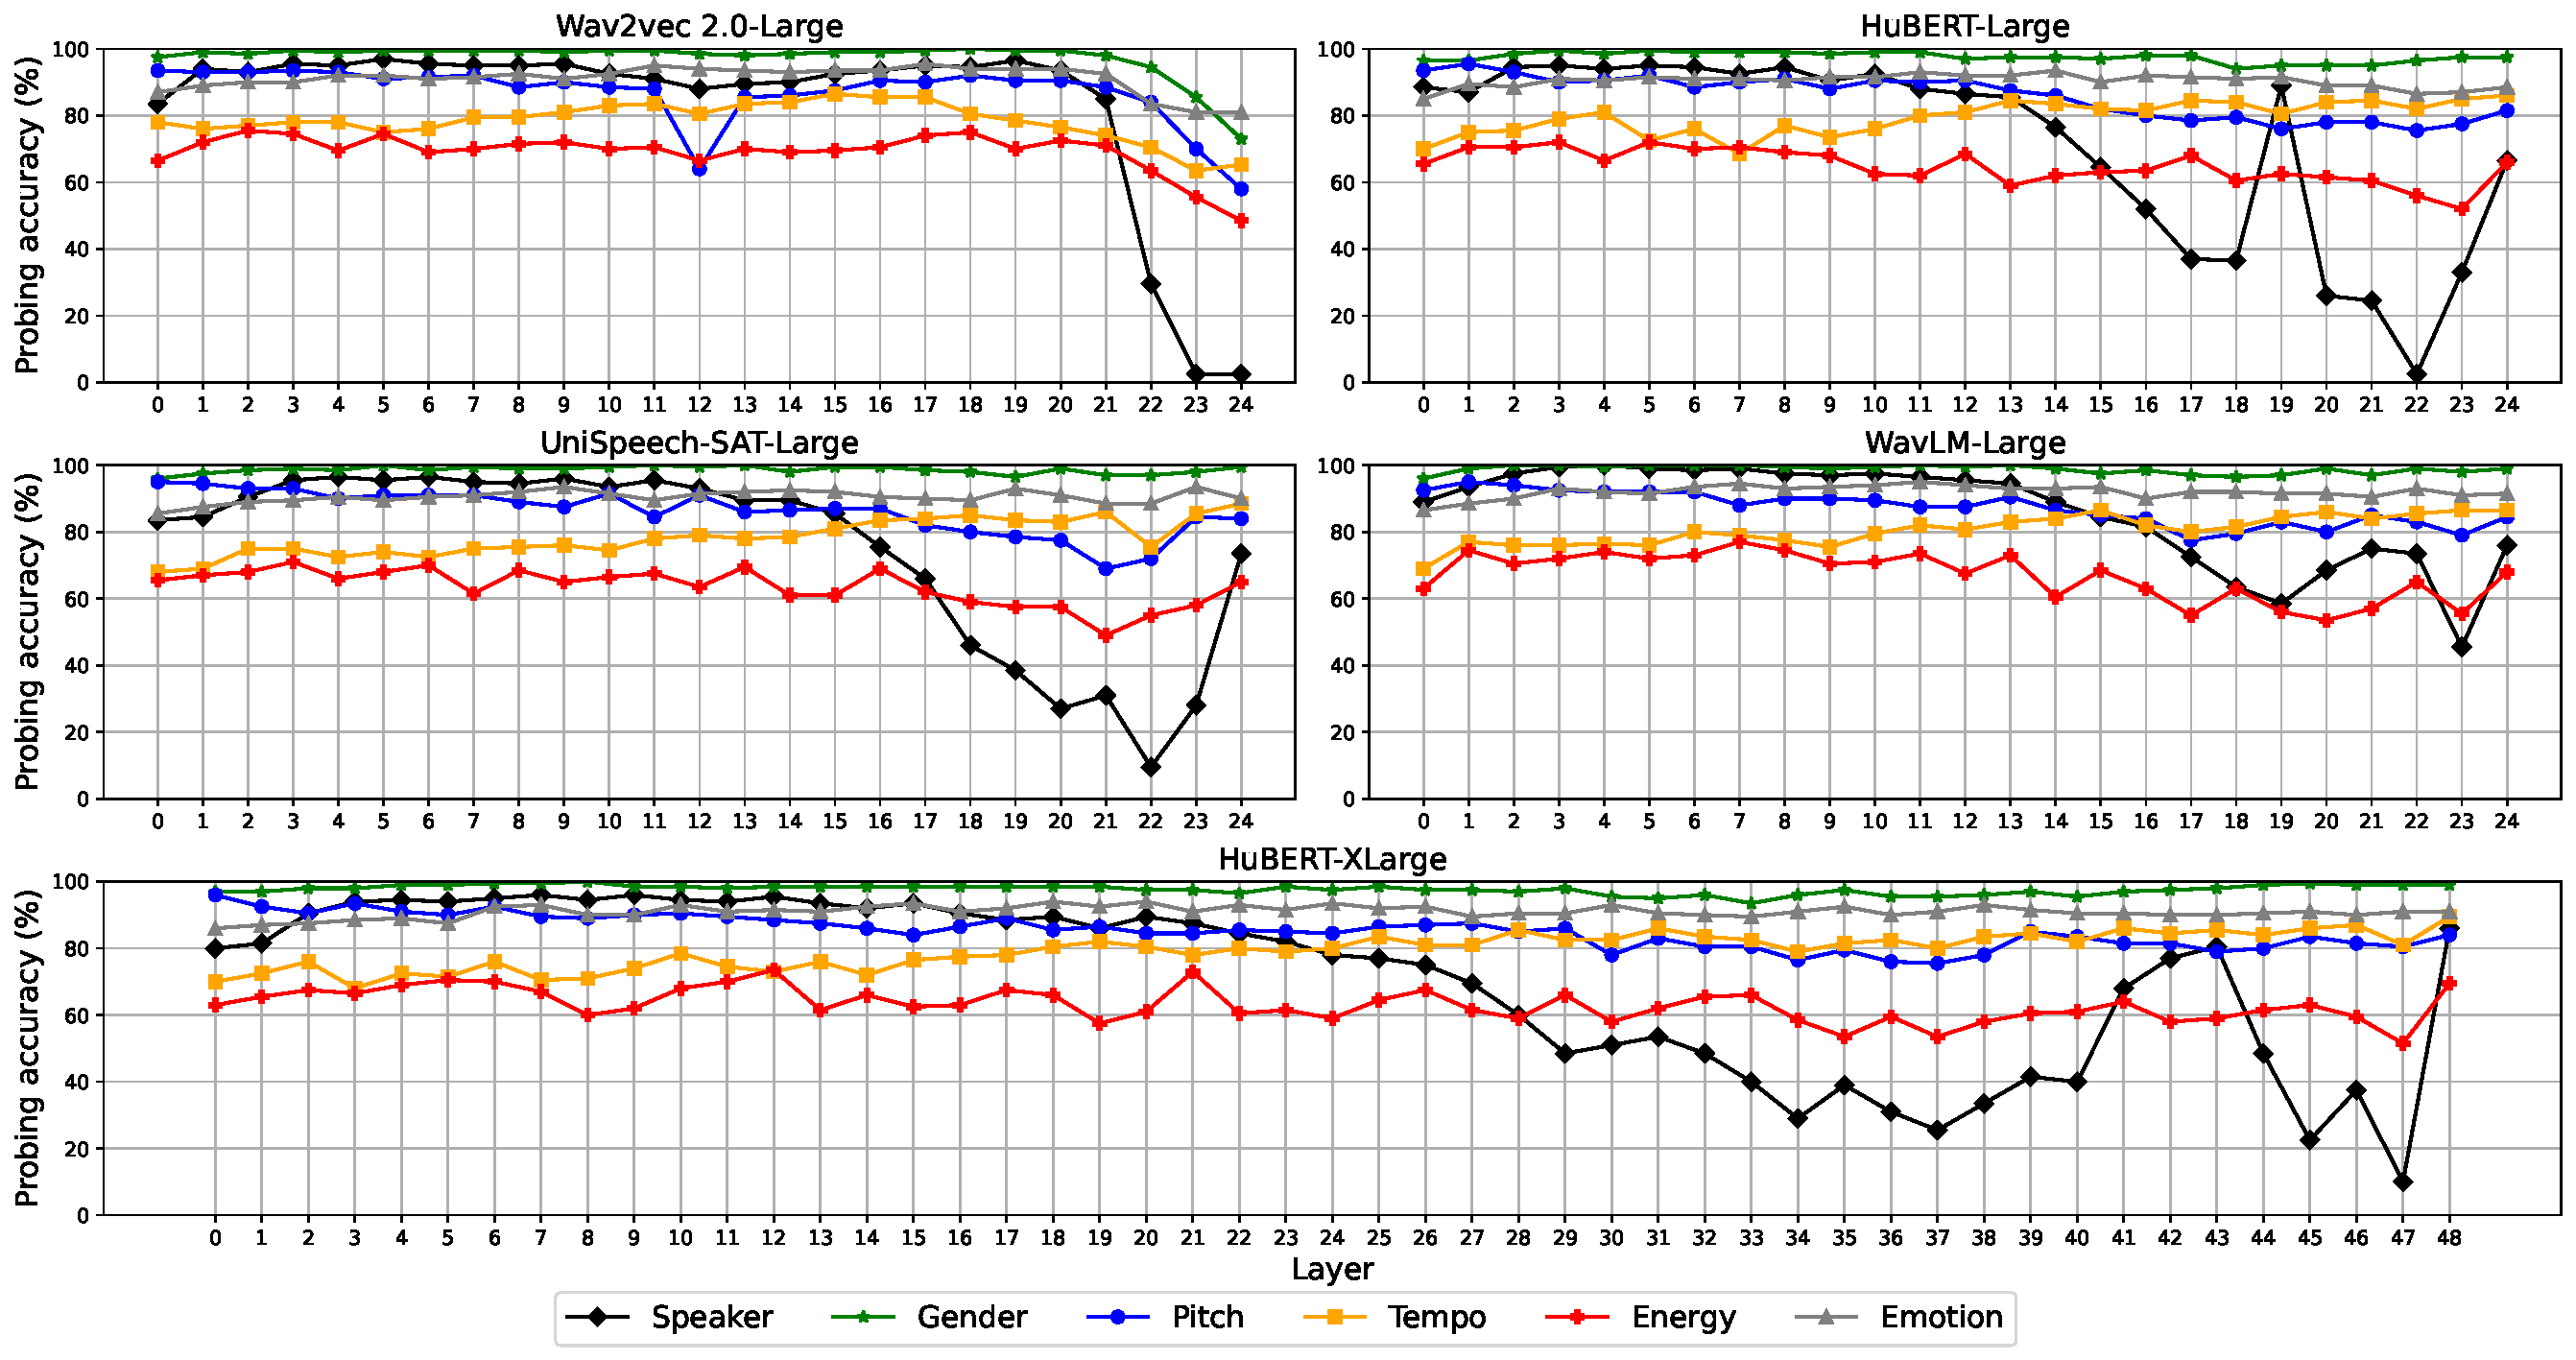
\includegraphics[width=\linewidth]{figures/Fig4.pdf}
  \vspace{-2em}
  \caption{Probing accuracies for the \textit{Large} and \textit{XLarge} variants of speech SSL models on the test set.}
\label{fig:large}
\vspace{-1.85em}
\end{figure*}


\subsection{Probed speaker-specific attributes}

\textbf{Speaker} identity and five speaker-specific features, categorised into three categories, are probed in this study: \textbf{Gender}, acting as a proxy for stable and long-term timbre quality features closely related to \textit{acoustic} characteristics; \textbf{Pitch}, \textbf{Tempo}, and \textbf{Energy}, representing three core dynamic attributes of \textit{prosody}; and \textbf{Emotion}, representing an affective state and \textit{paralinguistic} trait. In this study, Gender and Emotion are manually labelled. Pitch, Tempo, and Energy levels are derived from the dataset using acoustic processing tools, and each audio sample is labelled as ``High'', ``Normal'', or ``Low'' based on the overall distribution within the TextrolSpeech dataset~\cite{ji2024icassp}. Emotion labels include ``Happy'', ``Contempt'', ``Disgusted'', ``Angry'', ``Fear'', ``Surprised'', ``Sad'', and ``Neutral''.


\subsection{Models under investigation}

The intermediate representations from 11 pre-trained speech SSL models, sourced from \textit{Hugging Face}, are analysed. The selection covers four major model families at multiple scales to ensure the findings are generalisable:

\begin{itemize}
    \item \textbf{Wav2vec 2.0}: Wav2vec 2.0-\textit{Base}, \textit{Large}.
    \item \textbf{HuBERT}: HuBERT-\textit{Base}, \textit{Large}, \textit{XLarge}.
    \item \textbf{UniSpeech-SAT}: UniSpeech-SAT-\textit{Base}, \textit{Base-Plus}, \textit{Large}.
    \item \textbf{WavLM}: WavLM-\textit{Base}, \textit{Base-Plus}, \textit{Large}.
\end{itemize}

The \textit{Base} and \textit{Base Plus} models have 12 Transformer layers, outputting intermediate representations with 768 hidden states. \textit{Large} variants, comprising 24 Transformer layers, produce representations with 1,024 hidden states, while the \textit{XLarge} model has 48 Transformer layers with 1,280 hidden states.


\subsection{Training settings}

Following \cite{raj19asru}, cross-entropy loss is employed as the loss function for the classification tasks. The Adam optimiser is utilised with a learning rate of $0.001$. The batch size is set at $1,024$ and the model is trained for one epoch on the training set during each round. Mixed precision training is employed to accelerate the process.


\begin{table*}[t]
\centering
\caption{Peak test accuracies (\%, denoted as \textbf{Test}) with corresponding validation accuracies (\%, denotes as \textbf{Val}) and the specific layer (denotes as \textbf{L}) for all configurations. Layer 0 refers to the CNN encoder layer.}
% \vspace{-0.8em}
\vspace{-0.7em}
% \small
\resizebox{0.9875\linewidth}{!}{
\setlength{\tabcolsep}{3pt}

\begin{tabular}{@{}l *{6}{c c c}@{}}
\toprule
\multicolumn{1}{c}{\multirow{2}{*}{\textbf{Model}}} &
\multicolumn{3}{c}{\textbf{Speaker}} & \multicolumn{3}{c}{\textbf{Gender}} &
\multicolumn{3}{c}{\textbf{Pitch}}   & \multicolumn{3}{c}{\textbf{Tempo}}  &
\multicolumn{3}{c}{\textbf{Energy}}  & \multicolumn{3}{c}{\textbf{Emotion}} \\
\cmidrule(lr){2-4}\cmidrule(lr){5-7}\cmidrule(lr){8-10}\cmidrule(lr){11-13}\cmidrule(lr){14-16}\cmidrule(lr){17-19}
  & \textbf{L} & \textbf{Val} & \textbf{Test} & \textbf{L} & \textbf{Val} & \textbf{Test} & \textbf{L} & \textbf{Val} \textbf{}& \textbf{Test} & \textbf{L} & \textbf{Val} & \textbf{Test} & \textbf{L} & \textbf{Val} & \textbf{Test} & \textbf{L} & \textbf{Val} & \textbf{Test} \\
\midrule
Wav2vec 2.0-\textit{Base}           & 9  & 81.6 & 87.0 & 3  & 99.1 & 99.5       & 0  & 92.8 & 94.0        & 9  & 82.2 & 84.5        & 3  & 69.5 & 73.5        & 5  & 92.8 & 91.0 \\
HuBERT-\textit{Base}                & 4  & 71.7 & 78.5 & 3  & 98.7 & 99.0       & 0  & 92.0 & 94.5        & 11 & 82.2 & 84.5        & 11 & 66.0 & 69.5        & 6  & 91.9 & 90.0 \\
UniSpeech-SAT-\textit{Base}         & 0  & 81.3 & 84.0 & 7  & 98.2 & 99.0       & 1  & 92.3 & 95.0        & 11 & 83.9 & 86.0        & 2  & 67.2 & 68.5        & 11 & 91.4 & 89.0 \\
UniSpeech-SAT-\textit{Base-Plus}    & 0  & 77.9 & 76.0 & 3  & 98.9 & \best{100.0} & 0  & 92.5 & 94.0        & 11 & 86.5 & 87.0        & 1  & 67.2 & 71.5        & 8  & 92.3 & 90.0 \\
WavLM-\textit{Base}                 & 0  & 81.8 & 80.5 & 4  & 99.0 & 99.5       & 0  & 92.0 & 94.5        & 10 & 85.8 & 84.5        & 1  & 69.7 & 73.0        & 6  & 91.5 & 90.0 \\
WavLM-\textit{Base-Plus}            & 0  & 83.6 & 83.5 & 5  & 98.8 & \best{100.0} & 0  & 92.3 & 94.0        & 10 & 87.6 & 87.5        & 1  & \best{72.0} & 75.0        & 6  & 91.8 & 90.5 \\
\midrule
Wav2vec 2.0-\textit{Large}          & 5  & 94.9 & 97.0 & 18 & \best{99.4} & \best{100.0} & 0  & 93.0 & 93.5        & 15 & 86.4 & 86.5        & 2  & 70.5 & 75.5        & 17 & 94.8 & \best{95.5} \\
HuBERT-\textit{Large}               & 3  & 95.2 & 95.0 & 3  & 99.1 & 99.5       & 1  & 92.7 & 95.5        & 24 & 85.7 & 86.0        & 3  & 68.3 & 72.0        & 14 & 94.1 & 93.5 \\
UniSpeech-SAT-\textit{Large}        & 4  & 96.5 & 96.5 & 5  & 99.1 & \best{100.0} & 0  & 92.3 & 95.0        & 24 & 86.4 & 88.5        & 3  & 68.4 & 71.0        & 9  & 94.5 & 93.5 \\
WavLM-\textit{Large}                & 4  & \best{98.6} & \best{100.0} & 2  & 99.2 & \best{100.0} & 1  & \best{93.3} & 95.0        & 15 & 82.2 & 86.5        & 7  & 67.8 & \best{77.0} & 11 & \best{95.6} & 95.0 \\
\midrule
HuBERT-\textit{XLarge}              & 7  & 95.5 & 96.0 & 8  & 99.1 & \best{100.0} & 0  & 92.1 & \best{96.0} & 48 & \best{87.7} & \best{89.5} & 12 & 67.1 & 73.5        & 18 & 94.5 & 94.0 \\
\bottomrule
\end{tabular}
}
\vspace{-1.85em}
\label{tab:peak_results}
\end{table*}



\begin{table}[b!]
\vspace{-1.5em}
    \centering
    \caption{Probing accuracies ($\%$) of deep speaker embedding models on the validation (\textbf{Val}) and test (\textbf{Test}) sets.}
    \vspace{-0.7em}
    \label{tab:embed}
    \resizebox{\columnwidth}{!}{
    \begin{tabular}{ccccccc}
\toprule
\multirow{2}{*}{\textbf{Attribute}} &
\multirow{2}{*}{\textbf{Data}} &
E-TDNN & E-TDNN & ResNet & ResNet &
\multirow{2}{*}{CAM++} \\
& & 512 & 1024 & 34 & 293 & \\
\midrule
\midrule
\multirow{2}{*}{\textbf{Speaker}} & \textbf{Val} & 98.08 & 98.02 & \textbf{98.39} & 98.14 & 98.03 \\
                                   & \textbf{Test} & 98.50 & 98.50 & 98.00 & 98.50 & \textbf{99.00} \\
\cmidrule(r){1-2}\cmidrule(r){3-4}\cmidrule(r){5-6}\cmidrule(r){7-7}
\multirow{2}{*}{\textbf{Gender}} & \textbf{Val} & 99.41 & 99.42 & 99.53 & 99.48 & \textbf{99.71} \\
                                 & \textbf{Test} & \textbf{100.00} & \textbf{100.00} & \textbf{100.00} & \textbf{100.00} & 99.50 \\
\cmidrule(r){1-2}\cmidrule(r){3-4}\cmidrule(r){5-6}\cmidrule(r){7-7}
\multirow{2}{*}{\textbf{Pitch}} & \textbf{Val} & 85.70 & 83.71 & \textbf{86.31} & 84.04 & 86.12 \\
                                & \textbf{Test} & \textbf{86.50} & 81.00 & \textbf{86.50} & 79.00 & 84.50 \\
\cmidrule(r){1-2}\cmidrule(r){3-4}\cmidrule(r){5-6}\cmidrule(r){7-7}
\multirow{2}{*}{\textbf{Tempo}} & \textbf{Val} & 68.20 & 67.78 & 68.39 & 67.49 & \textbf{68.66} \\
                                & \textbf{Test} & 67.50 & 70.00 & \textbf{71.50} & 70.50 & 71.00 \\
\cmidrule(r){1-2}\cmidrule(r){3-4}\cmidrule(r){5-6}\cmidrule(r){7-7}
\multirow{2}{*}{\textbf{Energy}} & \textbf{Val} & 65.47 & 64.63 & 66.82 & 65.28 & \textbf{67.42} \\
                                 & \textbf{Test} & 63.50 & 63.50 & 66.00 & 66.50 & \textbf{67.00} \\
\cmidrule(r){1-2}\cmidrule(r){3-4}\cmidrule(r){5-6}\cmidrule(r){7-7}
\multirow{2}{*}{\textbf{Emotion}} & \textbf{Val} & 91.66 & 90.36 & 91.09 & 89.74 & \textbf{94.41} \\
                                  & \textbf{Test} & 88.50 & 88.00 & 87.00 & 84.50 & \textbf{93.00} \\
\bottomrule
\end{tabular}
    }
\end{table}

\section{Results and Analyses}


Figure~\ref{fig:base} illustrates the probing accuracy on the TextrolSpeech test data for the \textit{Base} and \textit{Base Plus} speech SSL models \cite{wav2vec2, hubert, unispeech-sat, wavlm} across different layers, while Figure~\ref{fig:large} demonstrates this for the \textit{Large} and \textit{XLarge} variants. A summary of peak probing accuracy for each attribute given by each model is illustrated in Table~\ref{tab:peak_results}.


\subsection{Hierarchy of attribute encoding}
\label{sec:hierarchical}

Despite differences in model architectures and pre-training data, all tested models exhibit a similar information hierarchy for processing speaker-specific attributes, consistent with the findings documented in the literature~\cite{ssl, yang2024taslp}.

The initial layers of those models function as powerful acoustic feature extractors. This is evidenced by \textbf{Pitch} and \textbf{Energy}, which consistently achieve their peak probing accuracies in the early layers before such information is abstracted away. \textbf{Gender}, acting as a stable acoustic attribute, maintains high probing accuracy across all layers. The probing accuracy curves for \textbf{Emotion} are also relatively stable from the initial to the final layers, indicating that the paralinguistic information is distributed almost uniformly across the network. The probing accuracies for \textbf{Speaker} are generally highest in the initial layers, suggesting that the shallow layers of the speech SSL models are optimal for speaker identification tasks.

The middle layers serve as a transitional stage, abstracting information and shifting the representations from the acoustic to the linguistic domain. The probing accuracy of \textbf{Tempo}, a prosodic feature highly correlated with linguistic content, continues to increase during this stage.

The final layers mostly exhibit clear identity suppression and content refinement. The probing accuracy for \textbf{Tempo} peaks at this stage, whereas the accuracy for \textbf{Speaker} steadily declines from the middle to the final layers. These results demonstrate that the final layers are primarily dedicated to refining speaker-invariant representations for content modelling. However, \textbf{Speaker} identify is unexpected recovered at the final layers of certain\textit{Large} and \textit{XLarge} models, which contradicts the prior consensus that speaker information is largely suppressed at this depth.


\subsection{Deconstruction of speaker identity in the representations}
\label{sec:deconstruction}

The probing results demonstrate that the ability of speech SSL models to identify speakers peaks in the early-to-mid layers, which aligns with the peak probing accuracies of \textbf{Gender}, \textbf{Pitch} and \textbf{Energy}. This suggests that these models identify a speaker by recognising their unique combination of foundational acoustic and prosodic patterns. Stable timbre features, including \textbf{Gender}, establish the basic voice quality, while dynamic \textbf{Pitch} provides the speaker's specific stylistic information.

The probing accuracies for \textbf{Energy} are constantly lower than those for features such as \textbf{Gender} and \textbf{Pitch}. Although its accuracy also tends to peak in the early layers, its lower overall performance suggests that energy is a less reliable or discriminative feature for speech SSL models.

\subsection{Model-specific variations and the impact of scale}

While the general information hierarchy is consistent across all models, the probing results reveal certain variations among different model families and scales.

For speaker-related tasks, models with pre-training objectives targeting noisy and multi-speaker environments, such as WavLM~\cite{wavlm}, are most successful. WavLM-Large achieves the highest or near-highest test accuracies across these attributes.

% This finding informs the design of a WavLM-Large-based voice timbre attribute detection (vTAD) system~\cite{chiu25vtad}.

However, analysing the models across different scales reveals an important trade-off. While larger models trained on more extensive datasets exhibit clear performance gains on complex high-level traits like \textbf{Speaker} and \textbf{Emotion}, improvements for fundamental acoustic and prosodic features are often marginal. This suggests that for downstream tasks requiring fine-grained manipulation of speaker-specific features, smaller and more efficient \textit{Base} or \textit{Base-Plus} models may offer sufficient performance and an improved performance-to-cost ratio. Conversely, tasks requiring high-level speaker or emotion modelling benefit significantly from larger-scale model variants.


\subsection{Ablation study}

To further understand the roles of model architecture and training data size in speaker modelling tasks, an ablation study is conducted by probing five variants of three popular deep speaker embedding models: ECAPA-TDNN (E-TDNN) ~\cite{ecapa-tdnn}, the ResNet-based $r$-vector~\cite{r-vector}, and CAM++~\cite{cam++}. These models, which have simpler architectures and are trained on a smaller VoxCeleb2 dataset~\cite{voxceleb2} specifically for SV, produce a single embedding vector. The five speaker embedding models are retrieved from \textit{WeSpeaker}~\cite{wespeaker}. The probing results are illustrated in Table~\ref{tab:embed}

As expected, the deep speaker embedding models achieve perfect probing accuracies for \textbf{Speaker} and \textbf{Gender} classification, confirming their high level of specialisation. Their probing performance on other \textit{prosodic} features and \textit{paralinguistic} traits, however, is lower than that of the speech SSL models. This suggests deep speaker embedding models heavily leverage voice quality information to distinguish between different speakers, but discard other stylistic details.

This comparison demonstrates that general-purpose speech SSL models learn richer and more discriminative representations of dynamic \textit{prosodic} and \textit{paralinguistic} features than models explicitly optimised for \textbf{Speaker} identity. Therefore, for downstream tasks requiring fine-grained analysis or control of \textit{prosody} and \textit{style}, the intermediate layers of large-scale speech SSL models are more capable than dedicated deep speaker embedding models.


\section{Limitations and Future Work}

This study is limited by the discretisation of continuous prosodic features into three levels and its reliance on TextrolSpeech annotations. This approach restricts granularity and may underestimate the richness of prosodic encoding. Furthermore, the use of a simple probing network presents a paradox: while low-capacity networks ensure interpretability by attributing performance to easily accessible information, they may fail to uncover information encoded a more complex ways. In contrast, more powerful probing networks could reveal hidden information, but they make it harder to determine whether classification success stems from the representation itself or the network's capacity. Future work will investigate this trade-off by comparing probing networks of varying complexities. Additionally, alternative datasets and fine-grained or regression-based probing methods could be explored. Developing more refined feature categorisations to address overlapping features, such as \textbf{Pitch} and \textbf{Tempo}, is another critical direction for future research.


\section{Conclusions}

% In this work, a large-scale probing analysis on multiple speech SSL models was conducted, demonstrating that these architectures learn complex hierarchical information from speech utterances. A detailed analysis of different speaker-specific attributes encoded in different scales of the models gives practical implications for model selection in specific downstream tasks.

To advance the explainability of speech SSL models, this study conducted a large-scale probing analysis across multiple model families and variants. This work maps how these models hierarchically learn and distribute complex information derived from speech. By deconstructing the layer-wise encoding of speaker-specific attributes across various model scales, this research translates hidden states into interpretable insights. While the observed information flow aligns with the literature consensus, the unexpected recovery of speaker-specific information in the final layers of certain speech SSL models is identified and analysed. This explainability analysis provides practical and transparent guidelines for selecting the most appropriate layer representations from speech SSL models for specialised speaker-related downstream tasks.


\section{Generative AI Use Disclosure}

The authors disclose that generative AI tools were utilised solely for the purpose of editing and polishing this manuscript, including correcting grammatical errors, refining sentence structures, and improving the overall clarity of the English text. All (co-)authors take full responsibility and accountability for the original research, data analysis, and technical content presented in the manuscript. No generative AI tool was used to produce any significant part of the manuscript.


\bibliographystyle{IEEEtran}
\bibliography{main}

\end{document}

%%% Local Variables:
%%% mode: LaTeX
%%% TeX-master: t
%%% End:
